% Type of the document is an article
\documentclass{article}

% use a graphics package for including images
\usepackage{graphicx}

% begin the document
\begin{document}

% give the document a title
\title{CS31310 Worksheet 1}

% list the author of the document
\author{Daniel Atkinson}

% print the title, author, etc... here
\maketitle

% start the abstract
\begin{abstract}

Automated Acceptance Testing using FitNesse and the FIT/Slim Frameworks

%end the abstract
\end{abstract}


\section{Setting up}
After setting up FitNesse with my install of java I ran it on port 8080 due to already running a webserver on the default port of 80 on the machine I use for assignments.
\begin{figure}[h]
\centering
	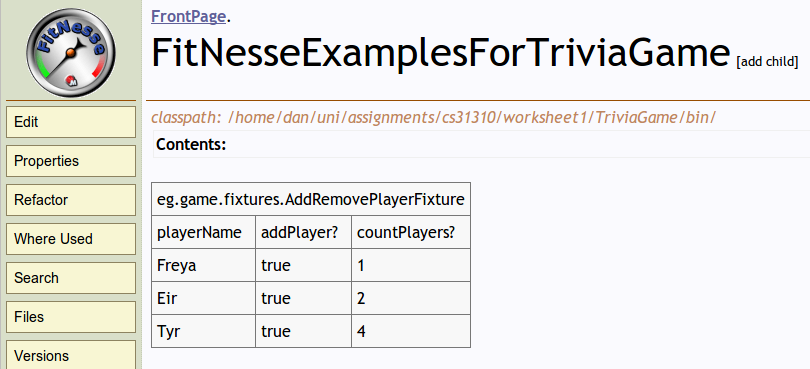
\includegraphics[width=5.0in] {figures/Screenshot1.png}
	\caption{Figure 1}
	\label{Adding players}
\end{figure}


\section{Running tests}
After setting up some sets using the wiki formatting I ran them under various levels of passing.
\subsection{Pass}
An example of passing all tests
\begin{figure}[h]
\centering
        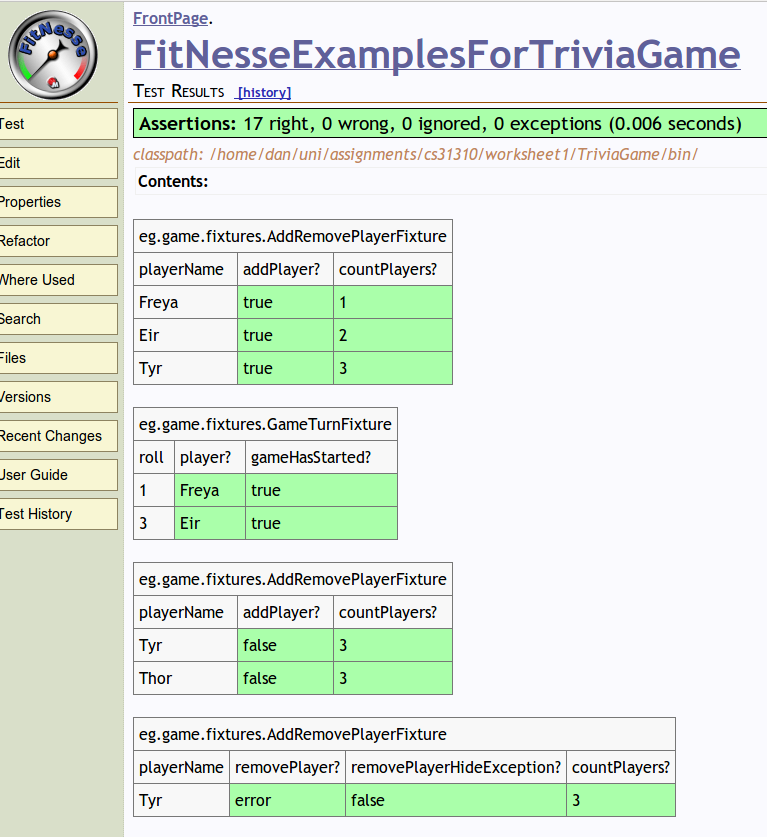
\includegraphics[width=3.0in] {figures/Screenshot2.png}
        \caption{Figure 2}
        \label{Pass}
\end{figure}

\subsection{Error}
An example of passing all test but one, which errors
\begin{figure}[h]
\centering
        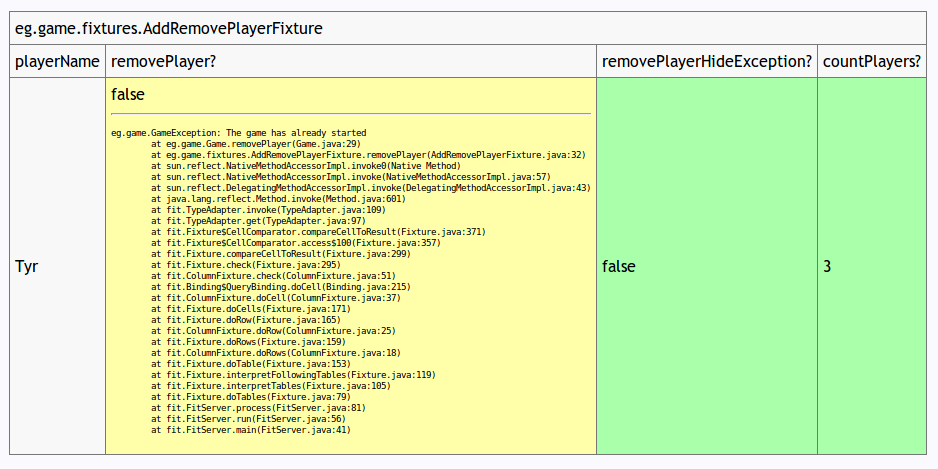
\includegraphics[width=3.0in] {figures/Screenshot3.png}
        \caption{Figure 3}
        \label{Error}
\end{figure}

\subsection{Fail}
An example of all tests passing apart from one which fails
\begin{figure}[h]
\centering
        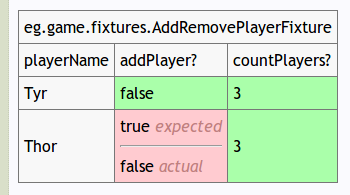
\includegraphics[width=2.0in] {figures/Screenshot4.png}
        \caption{Figure 4}
        \label{Fail}
\end{figure}


\section{Usefullness}
Tools such as FitNesse seem to be a usefull tool to allow non-developers to run their own test data against code.
\\This is not to say developers cannot also use this tool.  It does seem to make the tests more accessable.
\\Web front ends are a major focus of development currently, as they are standardised, to a point, cross platform as all you need to use them is a compatible web browser.  Having a compatable web browser is not an issue these days as all the major ones run on most platforms.
\\This is all nice and accessable, but, getting customers to actually create these test tables is a whole different matter.
\\Customers typicaly don't like doing extra work, thats what you are getting paid to do, so getting them to create these test tables will be a major task, then getting them to write usefull ones is even ahrder.  This is hindered even more, in the case of FitNesse, that they will have to write it in a wiki, just the fact that having to write things like "!|path.className|" etc... with extra syntax they may not be used to, it is more for them to learn.  Not all customers will be this way but enough to make this type of tool not worth using on the whole.
\\Like with any system there will be a number of cases where it will benefit the project, but it seems to have a flaw that it relies on people who may or may not have interest in doing th task or will just hand it off to somebody else which defeats the point of the system all together, which is to have the customer give quick feedback and 'direct' input into the system to aid agile development.




% end the document
\end{document}
